\section{Аналитический обзор программных продуктов, литературных источников}

\subsection{Общие понятия о навигации мобильных систем}

Навигация мобильных систем представляет собой процесс определения положения
устройства в пространстве и его перемещения в соответствии с заранее заданными
целями. Эта область охватывает множество технологий и методов, включая системы
позиционирования, карты и алгоритмы планирования маршрутов. Мобильные системы
могут быть использованы в самых разных сферах — от автономных транспортных
средств до мобильных роботов в промышленных и исследовательских приложениях.

Для навигации используются различные сенсоры для сбора информации о
своем окружении. Это могут быть камеры, лазерные дальномеры, ультразвуковые
датчики, IMU. Собранные данные обрабатываются с помощью
специализированных алгоритмов, что позволяет системе точно определять свое
положение и вносить изменения в маршрут в реальном времени. Успешная навигация
зависит от способности системы адаптироваться к изменениям в окружающей среде,
таким как перемещения других объектов, препятствия или изменения в маршруте.

\subsection{SLAM}

Для одновременной локализации и построения карты в мобильной навигации является
SLAM (Simultaneous Localization and Mapping — одновременное определение
положения и построение карты). Эта технология позволяет одновременно строить
карту окружающего пространства и определять свое местоположение относительно
этой карты, не имея предварительной информации о среде.

SLAM представляет собой не только способ построения карты, но и инструмент для
локализации — определения текущего положения системы в уже созданной карте. Это
особенно важно для мобильных роботов и автомобилей, которые не могут оперировать
в заранее определенных пространствах и нуждаются в создании карты окружающей
среды в процессе своего движения. Основная задача SLAM — это совместное решение
проблемы локализации и картографирования.

% Формальная постановка 

Задача SLAM заключается в вычислении оценки метоположения $x_t$ агента и карты
окрущающей среды $m_t$ из ряда наблюдений $o_t$ над дискретным временем с шагом
дискретизации $t$. Все перечисленные величины являются вероятностными. Цель
задачи состоит в том, чтобы вычислить $P(m_t, x_t | o_{1:t})$. Применение правила
Байеса является основой для последовательного обновления апостериорного
местоположения, учитывая карту и функции перехода~$P(x_t, x_{t-1})$:

\begin{equation}
P(x_t | o_{1:t}, m_t) = \sum_{m_{t-1}} P(o_t | x_t, m_t) \sum_{x_{t-1}} P(x_t |
	x_{t-1}) P(x_{t-1} | m_t, o_{1:t-1})
\end{equation}

Точно так же карта может обновляться последовательно:
\begin{equation}
P(m_t | x_t, o_{1:t}) = \sum_{x_t} \sum_{m_t} P(m_t | x_t, m_{t-1}, o_t)
	P(m_{t-1}, x_t | o_{1:t-1}, m_{t-1})
\end{equation}

Процесс SLAM можно разделить на несколько ключевых этапов. Сначала система
начинает с неопределенности относительно своей позиции и окружающей среды. С
помощью сенсоров она собирает данные о ближайших объектах, которые используются
для построения карты. На основе этой информации система оценивает, где она
находится, и корректирует свои вычисления с учетом новых данных. Постоянное
обновление карты и позиции позволяет системе поддерживать точность навигации,
несмотря на ошибки и неопределенности.

Помимо построения карты, мобильные системы навигации должны также учитывать
задачу нахождения маршрута между двумя точками на карте. Задача построения
маршрута должны учитывать габариты робота для создания маршрутов которые
возможно выполнить, а также высчитывать оптимальный маршрут на основе
пройденного расстояния и дистанции от ближайших препятствий.

Важной составляющей навигации является исполнение маршрута. Как только
оптимальный путь найден, система должна эффективно следовать этому маршруту,
корректируя свое движение при необходимости. Для этого используется целый набор
методов, включая управление движением, обработку сенсорных данных и системы
коррекции ошибок, избеганием препятствий. В процессе исполнения маршрута система
может столкнуться с различными непредсказуемыми ситуациями, такими как внезапное
появление препятствий или необходимость обхода объектов, что требует гибкости в
принятии решений.

Одной из главных сложностей в SLAM и навигации мобильных систем является работа
в динамических и изменяющихся условиях. Окружающая среда может быть не только
сложной и многообразной, но и динамичной — например, в случае движения других
объектов, изменения освещенности или появления новых препятствий. В таких
условиях мобильные системы должны постоянно обновлять свои карты и маршруты,
чтобы оставаться эффективными и безопасными. Это требует не только точных
сенсоров, но и быстрых алгоритмов обработки данных.

\subsection{Анализ существующих программных решений по теме дипломного
проектирования}

Программные фреймворки играют ключевую роль в разработке программного
обеспечения, предоставляя инфраструктуру для создания, тестирования и внедрения,
решая типовые задачи и позволяют сфокусироваться на разработке функционала
продукта. Однако, в области автономной навигации роботизированных платформ
многие разработки остаются закрытыми, что связано со спецификой определённых
проектов и их проприетарным характером. Несмотря на это, в индустрии широко
используется программное обеспечение с открытым исходным кодом.

В программировании роботов активно используются фреймворки для межпроцесного
взаимодействия между отдельными модулями\footnote{Под модулями подразумеваются
отдельные программы, являющиеся компонентами системы, исполняющиеся в отдельных
процессах операционной системы, или даже на отдельных компьютерах.}. Примером
таких фреймворков служат \ros{} и YARP.
Это позволяет разрабатывать ПО с использованием разных языков программирования,
осуществлять переиспользование отдельных модулей, анализировать и записывать
потоки сообщений, настраивать маршрутизацию сообщений.

\ros{} является де-факто стандартным фреймворком для программного обеспечения
роботизированных систем \cite{albonico2023software}. Основополагающая статья

\selectlanguage{english}
"Software engineering research on the Robot Operating System: A systematic
mapping study"
\selectlanguage{russian}
\cite{quigley2009ros} процитирована более
\num{13000} раз.

Yet Another Robot Platform (YARP) \cite{metta2006yarp} -- это фреймворк который
преследует цели, очень схожие с \ros{}. YARP поддерживает построение системы
управления роботом как набор программ общающимся в одноранговой сети используя
различные каналы связи, что по своей сути не отличается от целей ros{}. YARP
менее популярен и используется для более специализированных систем и не имеет
отличительных преимуществ, поэтому далее его не рассматриваем.

\ros{} это распределённый фреймворк из процессов (также известных как
\textit{ноды}), который позволяет разрабатывать исполняемые файлы индивидуально,
и свободно сочетать их во время исполнения. Эти процессы могут быть объединены в
\textit{пакеты} и \textit{стэки}, которыми можно легко делится и распространять.
\ros{} поддерживает единую систему кодовых \textit{репозиторириев} которые
позволяют сотрудничеству быть распределённым.

Философские цели \ros{} можно кратко сформулировать следующим образом
 \cite{quigley2009ros}:
\begin{itemize}
	\item P2P;
	\item Основанный на инструментах;
	\item Многоязычный;
	\item Тонкий;
	\item Свободный и открытый исходный код.
\end{itemize}

На данный момент существует две версии \ros{}: \ros{} 1 и \rosTwo{}. Первый
официальный релиз \ros{} (под кодовым названием ROS Box Turtler) состоялся 2
марта 2010 года. Первый официальный релиз \rosTwo{} состоялся 8 декабря 2017
года. \rosTwo{} это более расширенная версия \ros{}, спроектированная чтобы
устранить недостатки \ros{} 1, такие как: масштабируемость, производительность и
кросс-платформенная совместимость, используя Data Distribution Service (DDS) для
общения и вводя новые понятия, такие как жизненный цикл ноды и качество
обслуживания (QoS). Далее в дипломной записке при упоминании \ros{} идёт речь о
\rosTwo{}.

В экосистеме \ros{} есть готовый фреймворк для навигации -- Nav2
\cite{macenski2020marathon2}. Nav2 - это профессионально поддерживаемый преемник
навигационного стека ROS, в котором используются те же технологии, что и в
автономных транспортных средствах, уменьшенные, оптимизированные и
переработанные для мобильной и наземной робототехники. Этот проект позволяет
мобильным роботам перемещаться по сложным средам для выполнения заданных
пользователем прикладных задач практически с любым классом кинематики робота. Он
может не только перемещаться из точки А в точку Б, но и принимать промежуточные
позы, а также выполнять другие типы задач, такие как следование за объектом,
навигация по всему покрытию и т. д. Nav2 - это высококачественный навигационный
фреймворк промышленного уровня, которому доверяют более 100 компаний по
всему миру.


\begin{figure}[h]
\centering
	\fbox{
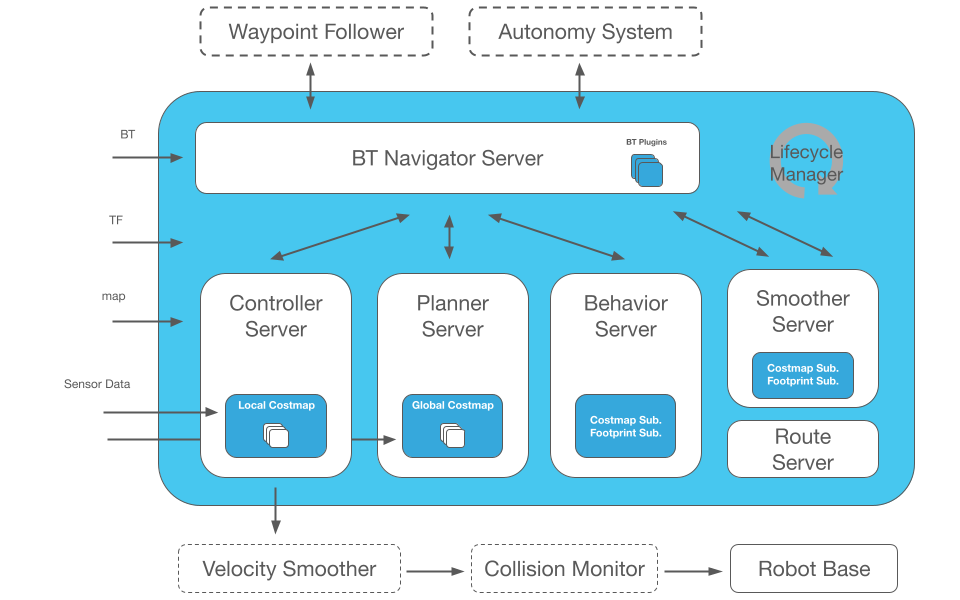
\includegraphics[width=14cm]{nav2_architecture}
}
\caption{Архитектура стэка Nav2}
\end{figure}

В Nav2 есть инструменты:
\begin{itemize}
	\item загрузки, обслуживания и хранения карт;
	\item локализации робота по предоставленной карте (SLAM предоставляет
		начальную карту);
	\item планирования полного пути через окружающую среду;
	\item управления роботом, чтобы он следовал по маршруту и динамически
		корректировался, чтобы избежать столкновений;
	\item сглаживания маршрутов, чтобы сделать их более непрерывными, плавными
		и/или выполнимыми.
	\item преобразование данных датчиков в модель окружающего мира;
	\item построение сложных и настраиваемых моделей поведения роботов с
		помощью деревьев поведения;
	\item выполнение заранее определенных действий в случае сбоя, вмешательства
		человека или других ситуаций;
	\item выполнение последовательных маршрутных точек, составляющих миссию;
	\item управление жизненным циклом программы и сторожевым таймером для
		серверов;
	\item простые динамически загружаемые модули для создания индивидуальных
		алгоритмов, поведений и т. д.
	\item мониторинг необработанных данных датчиков на предмет неминуемого
		столкновения или опасной ситуации;
\end{itemize}

\subsection{Анализ пакетов решающих задачу навигации, локализации и построения
карты}

Для навигации мобильной системы необходима карта, для построения которой
используют SLAM (Одновременную локализацию и построение карты). 

Алгоритмы SLAM можно разделить на две группы: более ранние алгоритмы,
использующие подходы, основанные на фильтрах Байеса , и более новые методы,
основанные на графах. Значимые реализации на основе фильтров, доступные в виде
пакетов \ros{} это: GMapping и HectorSLAM . Cartographer и KartoSLAM являются
основными доступными реализациями на основе графов \cite{macenski2021slam}.

Рассмотрим пакеты ros{}, такие как: SLAM Toolbox и GMapping:
\begin{itemize}
	\item SLAM Toolbox -- использует подход оптимизации
		графов.
	\item GMapping \cite{grisetti2005improving} -- использует Rao–Blackwellized
		Particle Filter (Фильтр частиц с использование теоремы Рао — Блэквелла —
		Колмогорова )
\end{itemize}

В SLAM Toolbox есть возможность делать почти всё, что есть в любой другой
платной и бесплатной библиотеке SLAM. Это включает в себя:
\begin{itemize}
	\item обычный точечный 2D SLAM для мобильных роботов (карта,
		сохранение pgm-файла) с утилитами, такими как сохранение карт;
	\item продолжение уточнения, перестройки карты или продолжения построения
		карты сохраненного (сериализованного) графа позиций в любое время;
	\item пожизненное картирование: загрузите сохраненный граф позиций и
		продолжайте строить карту, одновременно удаляя лишнюю
		информацию из новых сканов;
	\item режим локализации на основе оптимизации, построенный на основе
		pose-графа. Возможность запуска режима локализации без предварительной
		карты для режима «лидарной одометрии» с локальным замыканием контуров;
	\item синхронный и асинхронный режимы отображения;
	\item объединение кинематических карт (в разработке находится техника
		объединения манипуляций с эластичным графом);
	\item оптимизационные решатели на основе плагинов с новым оптимизированным
		плагином на основе Google Ceres;
	\item плагин RVIZ для взаимодействия с инструментами;
	\item инструменты манипулирования графами в RVIZ для манипулирования узлами
		и связями во время отображения;
	\item сериализация карт и хранение данных без потерь.
\end{itemize}

В то время как пакет GMapping предлагает обёртку над алгоритмом,
описанным в статье \cite{grisetti2005improving}, не включая дополнительный
функционал который предоставляется SLAM Toolbox, предоставляя лишь возможность
настройки параметров алгоритма и получения построенной карты.

\begin{figure}[h]
	\fbox{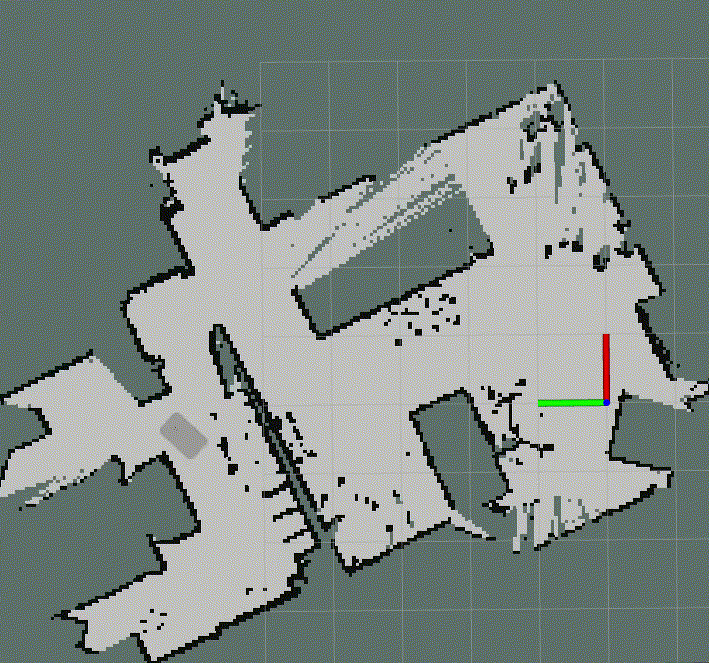
\includegraphics[width=7cm]{slam_toolbox_example}
\centering
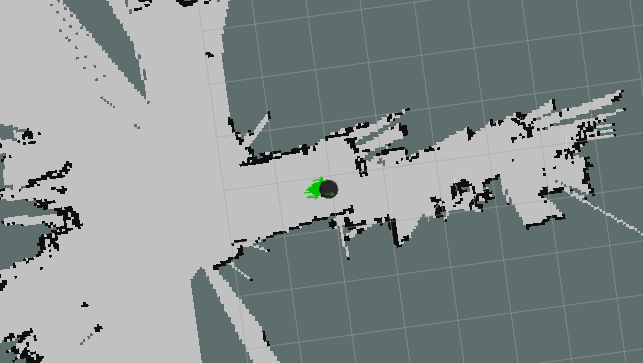
\includegraphics[width=7cm]{gmapping_example}
	}
	\caption{Пример построения карты используя SLAM Toolbox (слева) и GMapping
	(справа).}
\end{figure}

\subsection{Постановка целей и задач дипломного проектирования}
Фреймворки для разработки ПО для робототехники используют сервис для обмена
сообщения между модулями, но у этого архитектурного подхода есть ряд
недостатков: дополнительные затраты на сериализацию и десериализацию данных,
затраты на маршрутизацию сообщений, а также при использовании нескольких
программных модулей конечный программный продукт по своей сути является
распределённой системой, что вносит следующие недостатки:

\begin{itemize}
	\item проблемы с синхронизацией состояния, неконсистентность состояния;
	\item потеря сообщений;
	\item каскадный отказ системы;
	\item невозможность использования отладчика подключённого к одному
		исполняемому файлу для отладки всей системы навигации.
\end{itemize}

Исходя из этого, целью дипломного проектирования является разработка
программного средства осуществив вышеперечисленные оптимизации и устранив
вышеперечисленные недостатки, а также
реализовать необходимый набор функций, характерный для программных средств в
данной предметной области.

Для достижения поставленных целей следует решить следующие задачи: 
\begin{itemize}
	\item определить требования  к  разрабатываемому  программному  средству  и 
	составление спецификации, включающей их; 
	\item осуществить выбор  технологии  и  языка  программирования  для
		реализации программного средства; 
	\item провести проектирование архитектуры программного средства; 
	\item разработка алгоритмов для метода SLAM; 
	\item разработка алгоритмов для оценки местоположения; 
	\item разработка алгоритмов для поиска маршрута; 
	\item разработка алгоритмов для выполнения маршрута; 
	\item программирование и тестирование отдельных программных модулей; 
	\item тестирование готового программного средств.
\end{itemize}

